\hypertarget{group___c_m_s_i_s___core_debug}{}\section{C\+M\+S\+IS Core Debug}
\label{group___c_m_s_i_s___core_debug}\index{C\+M\+S\+I\+S Core Debug@{C\+M\+S\+I\+S Core Debug}}
Collaboration diagram for C\+M\+S\+IS Core Debug\+:\nopagebreak
\begin{figure}[H]
\begin{center}
\leavevmode
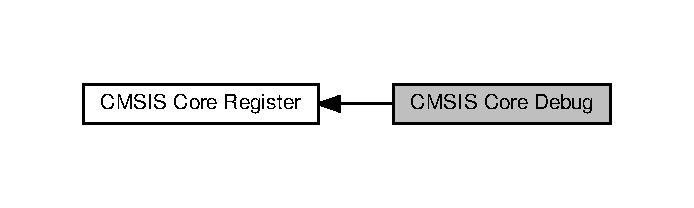
\includegraphics[width=333pt]{group___c_m_s_i_s___core_debug}
\end{center}
\end{figure}
Cortex-\/\+M0 Core Debug Registers (D\+CB registers, S\+H\+C\+SR, and D\+F\+SR) are only accessible over D\+AP and not via processor. Therefore they are not covered by the Cortex-\/\+M0 header file. 